\section{Improving generators}
Generators are obtained by using the $\epsilon$-constraints method which is one of the well-known scalarization techniques \cite{Chankong1983MultiobjectiveDM} aimed at getting a sample of efficient solutions of a MOLP. Those generators form an efficient set for the relaxed problem. That is to say, the set of all generators is also the lower bound set $L$. Since GM starts the search based on each $k$-th generator, one would like to have a better initial solution in order to reach a feasible solution faster.

\subsection{Bugs in Gravity Machine}

\subsubsection{Generators not feasible}
The previous version of Gravity Machine did use the GLPK solver to generate the lower bound set by the $\epsilon$-constraints method. 
However, closer to the line passing through the Nadir and the origin the more constrained the MILP representing the current generator. 
Since considered problems have lot of constraints and variables some numerical issues may arise \cite{gurobiNumIssues}. Infeasibility hence
may appear during the solving process for problems which has at least one (feasible) optimal solution. In addition, the \textit{Julia} wrapper
for GLPK seems to be known for returning the solution minimizing constraints violation\footnote{\url{https://discourse.julialang.org/t/access-infeasible-optimization-results-glpk-with-semicontinuous-variable/59972}}.
Finally, as the termination status was not correctly handled, some generators turn out to be used whereas there were not "trully" feasible.
\paragraph*{Patch:}
The termination status is now considered and GM properly fails if a generator is not feasible. 
Tolerance attribute was hand-tuned to allow the solver to find a feasible solution. \noteErwan{ça serait bien que ce ne soit pas "hand-tuned" \url{}https://discourse.julialang.org/t/scalling-both-primal-and-dual-feasibility-tolerance-according-to-the-size-of-the-problem/97455}.
It is worth noticing that no difference in the performance has been observed. The robustness is the matter here.
In addition, GLPK was replaced by HiGHS~\cite{highs}. Indeed, the latter shows better performances than GLPK~\cite{bench_solver} and is still open-source.

\subsubsection{Soft conic constraints $\lambda_1$ and $\lambda_2$}
Both vectors $\lambda_1$ and $\lambda_2$ were accidentaly swaped in their definition such that the "guidance mechanism" was useless and a fortiori misleading.

\subsection{Empirical findings}
Empirical evidences tend to show that very few variables are set to non-integral value for each generator.
%TODO

\subsection{Setting some variables binary}
At first sight, non-solved to integrality variables should be set binary and the problem re-optimized. The latter allows GM to find initial solution Then, a generator closer to $Y$ should result from a the re-optimization process. However, several issues arises:

\subsubsection{Communicating vessels effect}
Since not all constraints are set binary, some variables found to be zero or one might become fractional. 
A number of variables found fractional after the second stage solving greater than the number of variables found fractional after the first stage solving represents the worst case. 
As far as our experimental results show us, this situation is very rare. \noteErwan{à reformuler}
%TODO
\subsubsection{Same generators lead to the same solution}
Ideally, one would that each generator $\bar{y}^k$ converges to a different $\Tilde{y}^{k,t}$ for some iterations $t\in \mathbb{N}$.
Below, we consider $J_0(x)$ (and $J_1(x)$) the set containing the index of variables set to zero (respectively to one) into the solution $x$.
Some well known modelization techniques are briefly presented and their pertinence for GM is studied. For the major part of them, 
they are inspired by canonical cut constraints introduced by~\cite{canonical_cut} and used for the same purpose by~\cite{Hanafi2011}.

\paragraph*{Canonical cut constraint:}
\begin{proposition}\label{bincutconstraintexact}
    Let $x^0$ be a vector in $\set{0,1}^n$. The following inequality
    \begin{equation}
        \sum_{j\in J_1(x^0)} x_j + \sum_{j \in J_1(x^0)} 1-x_ j \geq 1
    \end{equation}
    cutts off solution $x^0$ without cutting off any other solution in $\set{0,1}^n$.
\end{proposition}
\begin{proof}
Let's suppose that $x^0$ is not cutted off by the constraint. Then $x = x^0$ implies $0\geq 1$ from (1). The cutting off is proved.
\\Finally, a solution $x^1 \neq_1 x^0$ is assumed to be cutted off by the constraint. That is to say
\begin{align}
    & \sum_{j\in J_1(x^0)} x_j^1 + \sum_{j \in J_1(x^0)} 1-x_ j^1 = 0 \\
    \Longleftrightarrow &   \| x^0 - x^1 \| = 0
\end{align}
In other words $x^0 = x^1$ and $x^0 \neq x^1$ which is impossible. Then,~\ref{bincutconstraintexact} holds.
\end{proof}
\begin{proposition}
    Gravity Machine does not longer guarantee the rectitude of $L$ if $x^0\in \left\lbrack 0,1 \right\rbrack ^n$
\end{proposition}
\begin{proof}
    We exhibit a counter-example. Let be a $1$-01LP of the form:
    \begin{align}
        \text{Min}  & \quad x_1 + x_2\\
        s.t & \quad x_1 + x_ 2 \geq \frac{1}{4}\\
        & -x_1 + x_2 \geq -\frac{3}{4}\\
        & x_1, \: x_2 \in \set{0,1}
    \end{align} 
    According to~\ref{fig:counterExampleL}, $x^* = \left(0,1\right)$ is clearly the optimal solution whereas 
    the optimal solution for the relaxed problem is $x^0 = \left( 0, \frac{1}{4}\right)$.
    Since, $x_1$ has a continuous value, only $x_2$ is present in the new constraint:
    \begin{equation}
        1-x_2 \geq 1 \Leftrightarrow x_2 = 0
    \end{equation}
    Consequently, this new constraint prevent the solver finding the $x^*$ and what is more make the problem infeasible.
\end{proof}
\begin{figure}
    \centering
    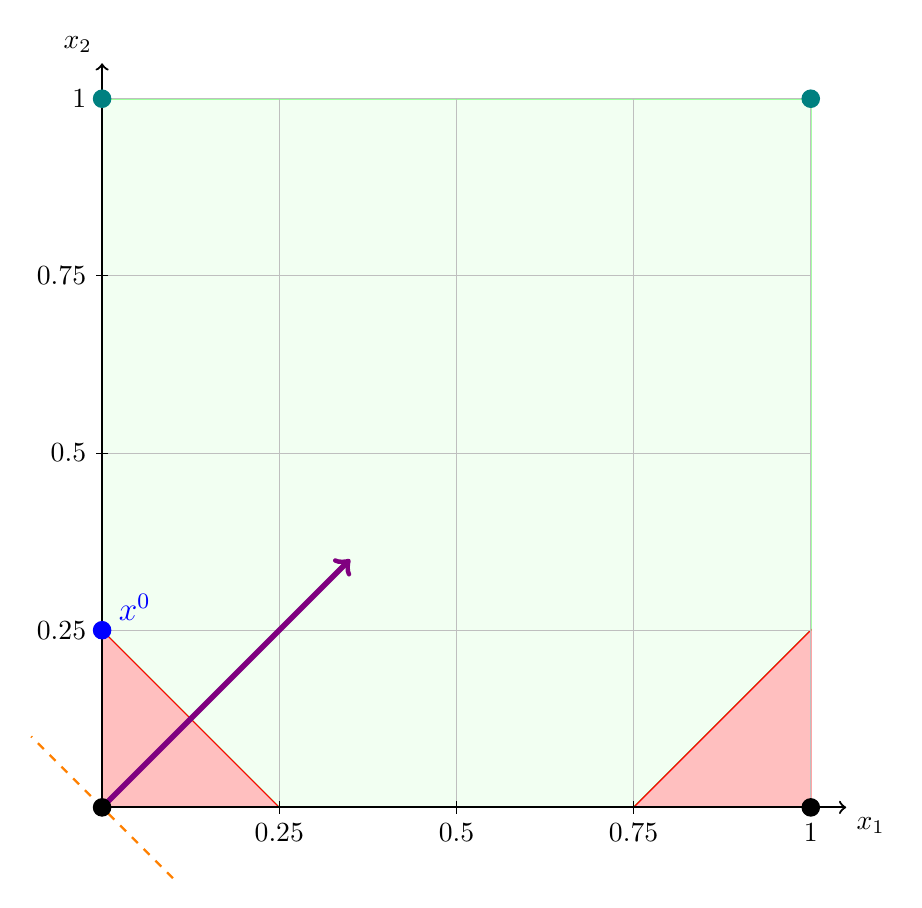
\begin{tikzpicture}[scale=9]
        \filldraw[fill=green!5,draw=green] (0,0.25)--(0,1)--(1,1)--(1,0.25)--(0.75,0)--(0.25,0)--cycle;
        \filldraw[fill=red!25,draw=red] (0,0)--(0,0.25)--(0.25,0)--cycle;
        \filldraw[fill=red!25,draw=red] (1,0)--(1,0.25)--(0.75,0)--cycle;
        \draw[step=0.25cm,color=gray!50] (0,0) grid (1,1);
        \foreach \x in {0.25,0.5,0.75,1}{
            \draw (\x cm, 0.25pt) -- (\x cm,-0.25pt) node[anchor=north] {$\x$};
        }
        \foreach \y in {0.25,0.5,0.75,1}{
            \draw (0.25pt, \y cm) -- (-0.25pt,\y cm) node[anchor=east] {$\y$};
        }
        \draw[thick,->] (0,0)--(1.05,0) node[anchor=north west] {$x_1$};
        \draw[thick,->] (0,0)--(0,1.05) node[anchor=south east] {$x_2$};
        \draw[->,violet,line width=2pt] (0,0)--(0.35,0.35);
        \draw[orange, dashed,thick] (0.1,-0.1)--(-0.1,0.1);
        \foreach \x/\y in {0/0, 1/0}{
            \filldraw[black] (\x,\y) circle (0.35pt);
        }
        \foreach \x/\y in {0/1, 1/1}{
            \filldraw[teal] (\x,\y) circle (0.35pt);
        }
        \filldraw[blue] (0,0.25) circle (0.35pt);
        \node[above right,blue] at (0.01,0.25) {\large \textbf{$x^0$}};
    \end{tikzpicture}
    \caption{Illustration of the counter-example}\label{fig:counterExampleL}
\end{figure}
\paragraph{Cones}

\begin{algorithm}
\caption{Improving generators}\label{alg:Generators_improvement}
\KwData{$L$,$\lambda_1$,$\lambda_2$,$\tau$,$\alpha$}
\KwResult{$L_I$,$U$}
\Begin{
 $L,F \gets \textsc{ComputeGenerators}(\mathcal{D},n_L)$\;
 \ForAll(//each $k$-th unfeasible gen){$z(\bar{x}^k)\in L,\Bar{x}^k\notin F$}{
  
 }
 }
\end{algorithm}
\subsubsection{Too much binary variables increase the solving time}
As shown by our empirical data, less than 20

\section{Improving projection}
By the same token as the generators improvement, the projection used during GM can be improved by adding some integrity constraints on the non 

